\chapter{Background}
\label{ch:background}
What belongs to biolinguistics, what do we know about the vocal capabilities of the bat \emph{S. bilineata} and how is this connected to \gls{ml}. This and many more insights are provided throughout this chapter.

\section{Biolinguistics}
More than anything else, language defines human nature. Language allows infinite expression with finite means \cite{Hauser2002Neuroscience:Evolve} enabling us to exchange ideas and transmit knowledge across generations, building the foundation of our technological advances and cultural heritage. However, the origins of language remain a puzzle, possibly the most challenging in science because language does not fossilize \cite{TecumsehFitch2010TheLanguage}. This renders tracing the evolution of language extremely challenging. The current most promising approach to solve this puzzle is to comparatively investigate the biological foundations of language across species \cite{Fitch2018TheAnalysis}.

The biolinguistic approach combines research methods from fields such as neurogenetics, animal behaviour, linguistics, developmental psychology, bioinformatics and mathematics to understand the underlying mechanisms and processes of human language. This make sense, as language itself is a complex system composed of several key factors (e.g. syntax, semantics, vocal imitation) and various cognitive abilities (e.g. social learning, theory of mind, recursive processing) \cite{Fitch2010SocialPhylogenies}.
Although no non-human animal communication system equivalent to the human language exists, bioacoustic research demonstrated that non-human animal vocal communication can be complex in terms of vocal repertoire size (i.e. the number of distinct syllables) (e.g. bats: \cite{Behr2004}; songbirds: \cite{Eens1989TemporalStarling}; cetaceans: \cite{Payne1971SongsWhales}), syntactical rules (i.e. the rules according to which the acoustic units – for example syllables - are arranged within vocal sequences; \cite{Weiss2014})  and vocal versatility (i.e. vocal plasticity allowing to modify existing signals and/or learning new signals from scratch based on social experience) \cite{Wirthlin2019ATrait}. Furthermore, non-human animals possess multiple cognitive skills which are required for language acquisition in the first place, such as associative learning, vocal imitation and joint attention \cite{Fitch2010SocialPhylogenies}. Therefore, the biolinguistic research in non-human animal vocal communication aims to understand if and to what extent key features and cognitive skills evolved compared to our own.

\section{Vocalisation}\label{sec:vocalisation}
Across many species, vocal communication is a common social behaviour.
Bioacoustic research seeks to uncover the structure, mechanism, behaviour and reason for vocal communication. This includes how signals are generated and perceived and how information about identity, fitness, presence of danger, environmental stress and possibly much more is transmitted. In the same way, the extent to which fitness and reproductive success are influenced by communication, is also of interest \cite{Kershenbaum2016, Manteuffel2004}.
This list is not exhaustive, thus as one can imagine, there is a large amount of unanswered questions in this field.
Unfortunately, only a tiny fraction of vocal communication seems to have been studied in detail so far. Here, the challenging work of segmenting acoustics into temporally discrete units and classifying them correctly according to specific characterising properties plays a major time-consuming, yet crucial role.

When it comes to vocal learning in non-human animals, the research field seems to be quite limited with focus on birds \cite{Petkov2012} and evidence in mammals centered around cetaceans \cite{Janik2014}, pinnipeds \cite{Reichmuth2014}, elephants \cite{Poole2005} and bats \cite{Knornschild2014}.
In recent years, researchers are debating about understanding vocal learning as a continuum rather than a dichotomy (absent vs present), including not only vocal imitation but also vocal plasticity, including the modification of innate calls based on social experience.
Martins et al. discuss the concept of a wider vocal learning continuum including more vocal abilities which are now being uncovered in other species.
Thus engaging a broader comparative study about vocal learning, as the current view seems to be too narrow and excludes vocal abilities \cite{Martins2020VocalContinuum}.

Still, non-human mammalian species which possess the ability of vocal imitation (i.e. learn a vocalisation from scratch based on the auditory input from a tutor) are especially promising candidates to study mechanisms and processes involved in language learning. Vocal imitation is a mandatory capacity for human babies and infants to acquire speech (i.e. oral output of language) \cite{Vihman2014}. One of the most important first steps in human infant speech acquisition is the canonical babbling phase during which infants acquire the phonological repertoire of the maternal language \cite{OLLER1980THEINFANCY,Vihman2014}. Infants imitate the basic speech sound subunits (i.e. consonant-vowel syllables) and refine their oral output and control over speech articulators by rehearsing syllables in sequences (e.g. "mamama", "bababa") \cite{Kuhl1996}.

\section{Vocal communication of the greater sac-winged bat}
\begin{figure}[H]
\centering
  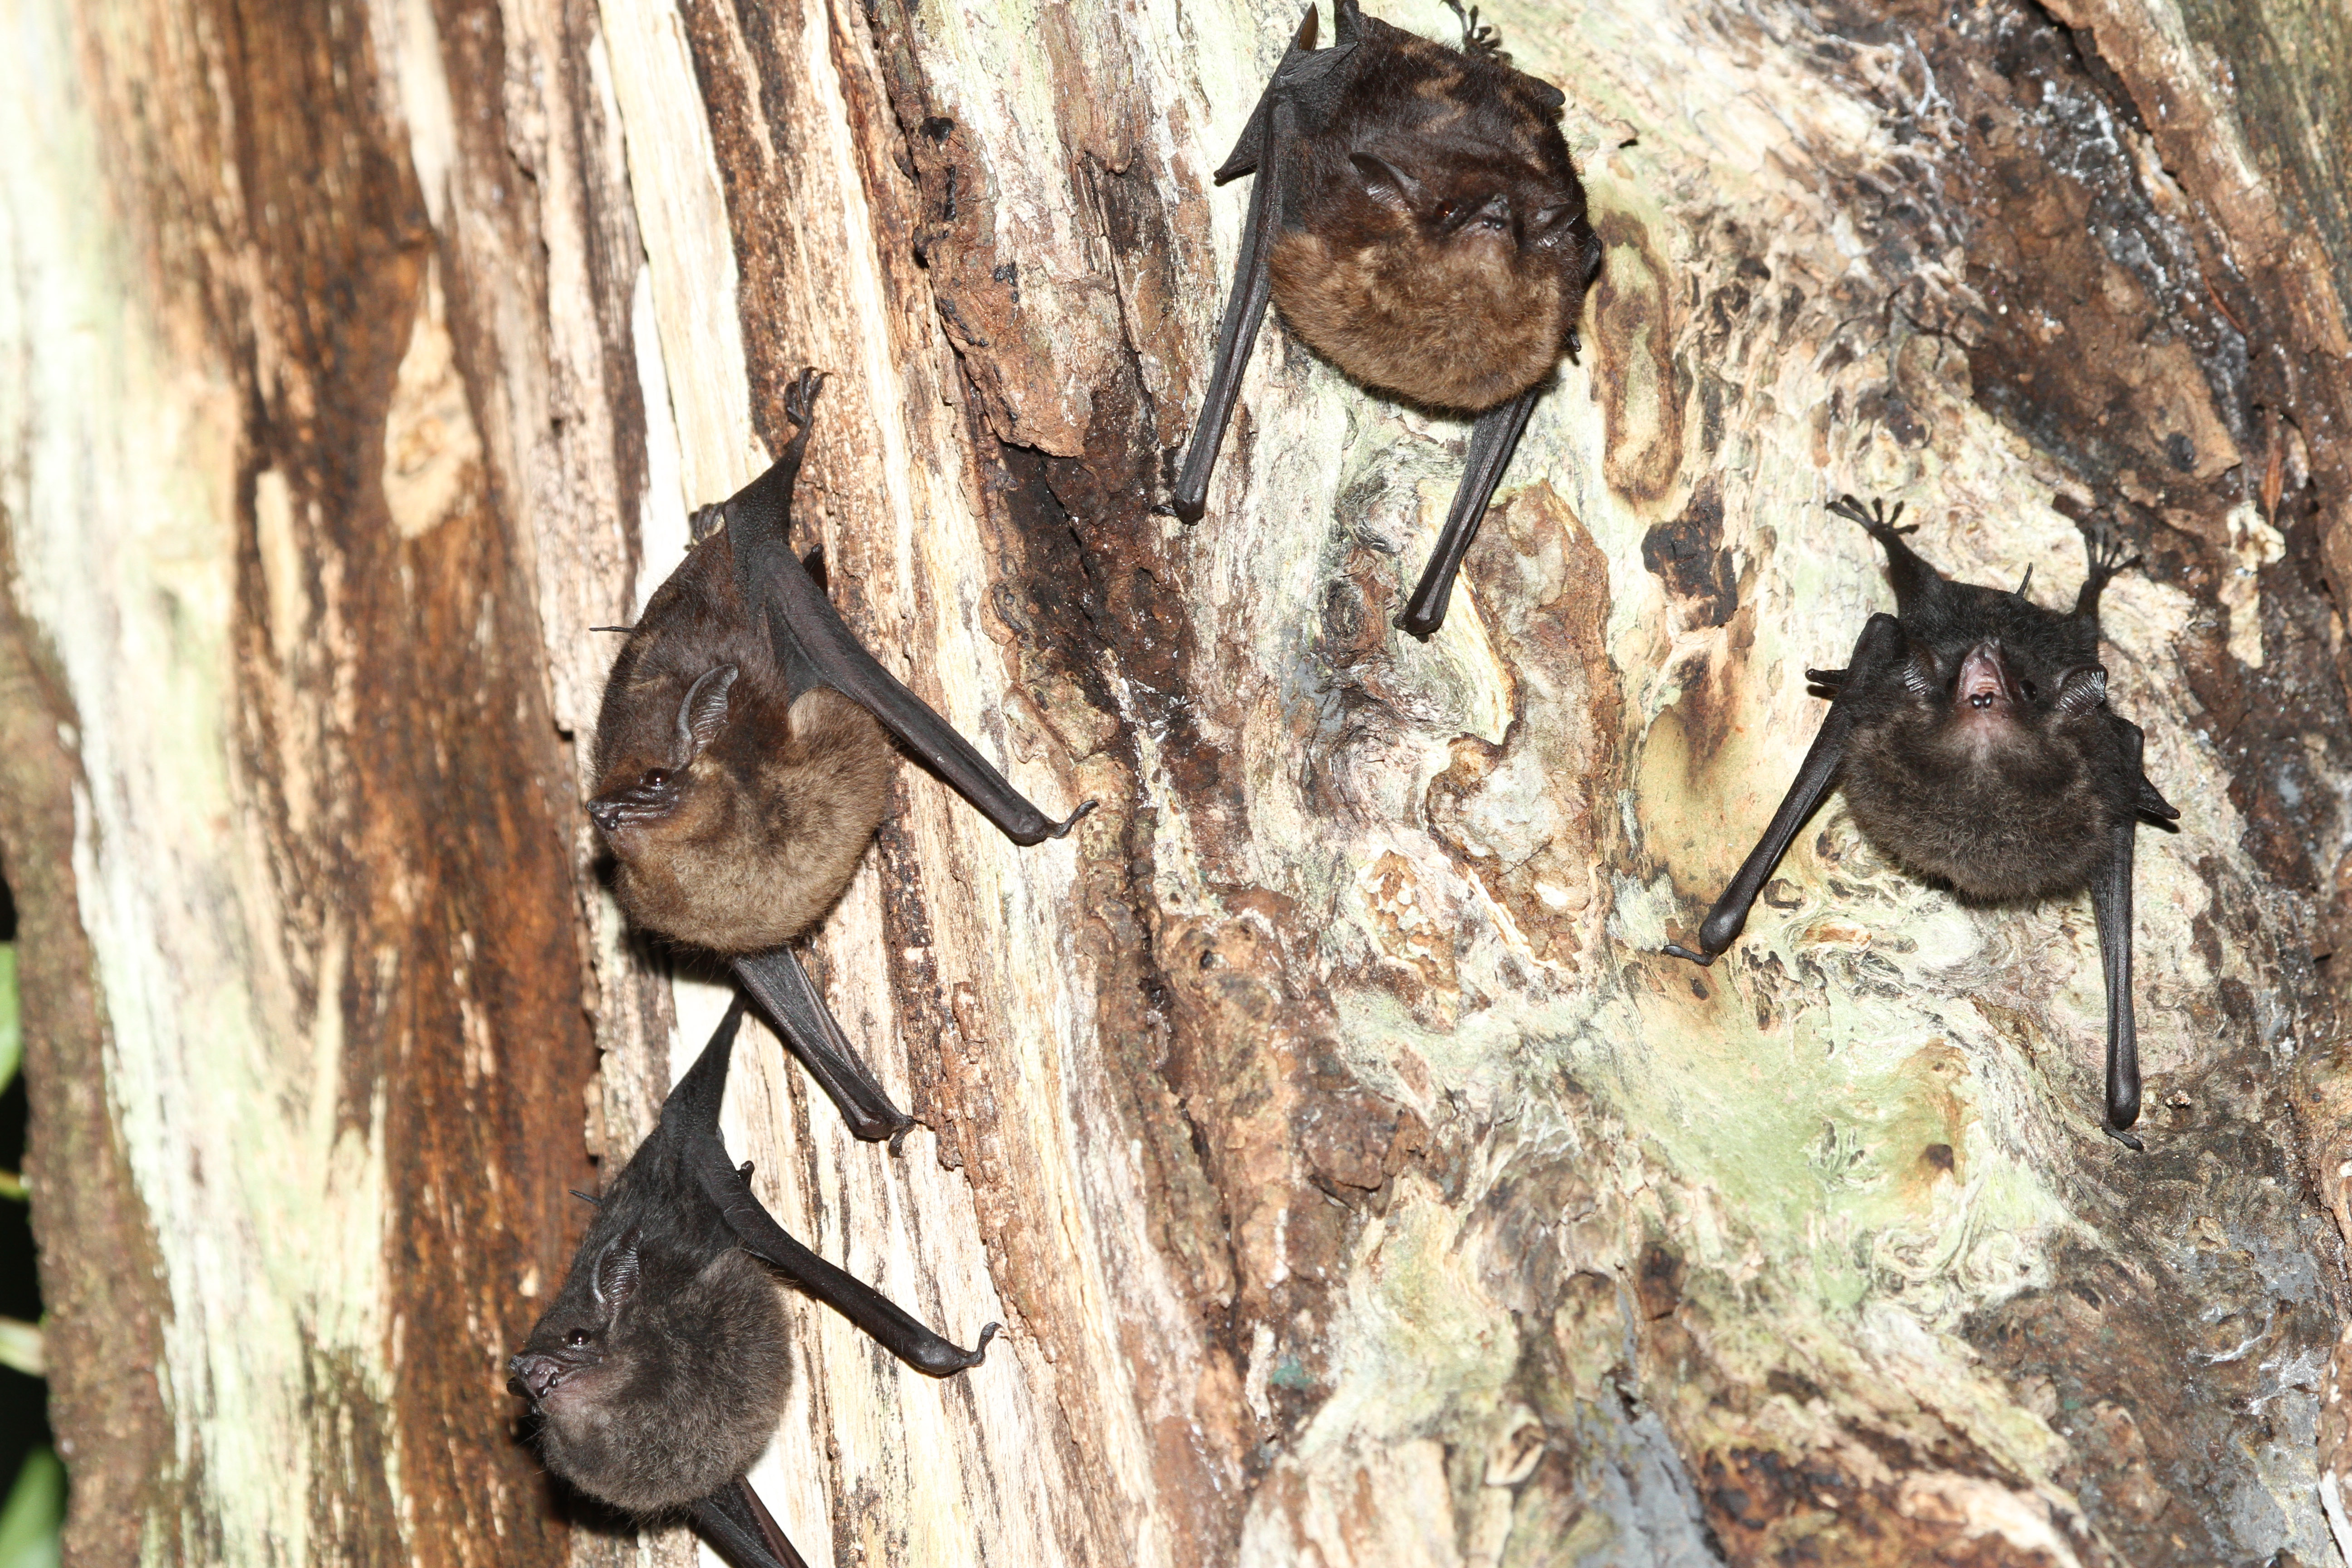
\includegraphics[width=0.7\textwidth]{image/Sacco Dayroost.jpg}
  \caption{Greater sac-winged bats (\emph{Saccopteryx bilineata}) roosting in their day roost, the young one on the right is vocalising. The smaller bats with the dark fur are juveniles and the others with lighter fur are their mothers. (© Michael Stifter)}
  \label{fig:sacco}
\end{figure}

A highly promising candidate for comparative biolinguistic studies is the neotropical bat species \emph{Saccopteryx bilineata}.
This bat species is a vocal production learner (i.e. capable of vocal imitation) \cite{Knornschild2010} and possesses a large vocal repertoire including two song types produced by adult males \cite{Knornschild2006}. During ontogeny, pups produce long vocal sequences composed of precursors of syllable types of the adult repertoire mixed with pup-specific vocalisations. While babbling, pups acquire a part of the adult vocal repertoire through vocal imitation, namely the syllables of the territorial song \cite{Knornschild2006}. For several weeks, the precursors of the territorial song syllables gradually converge towards the territorial song of tutor males, irrespective of relatedness and pup sex \cite{Knornschild2010}.
Studying the vocal practice behavior of pups offers the opportunity to study the underlying mechanisms crucial for vocal imitation because babbling represents the oral output of ongoing learning processes. Hence, investigating acquisition of learned territorial song syllable types could serve to unravel shared mechanisms and key factors across mammalian vocal learners including humans.


\section{The value of syllable type classification}\label{sec:syllable_classification}
% more about features, which features are taken for manual classification -> methos
To gain insight about potential information encoded in acoustic vocalizations, besides behavioural observations accompanying social vocalizations to infer the context, acoustic measurements are used.
Acoustic measurements can be taken over the entire vocalization (e.g. over an entire multisyllabic call) and from acoustic units such as syllables. In general, syllables are defined as continuous sound surrounded by silence.
To measure syllables it is necessary, to detect, label and sometimes classify them.
Currently, measuring and analysing syllables in vocal sequences is an extremely time-consuming job worked out mostly manually with the assistance of audio analysis tools.
Additionally, the missing knowledge about how animals perceive vocalizations (e.g. what is the smallest meaningful acoustic unit) makes the acoustic analysis challenging. Usually, syllabic units are defined based on information of the oscillogram and spectrogram. Then, possible information encoded in vocalizations can be inferred from accompanying behavioural observations.

% Additionally, the missing knowledge about the inner processing of the auditory system of the target animals requires expert knowledge about the vocalisation and their inherent physical features, resulting in classifying the syllables on a mathematical physical basis, which then could be connected to social behaviours in additional monitoring studies.

One aspect of understanding vocal learning processes in \emph{S. bilineata} involves analyzing the acoustic parameter change of territorial song syllables across ontogeny.
This begins with the selection of these particular syllable types within babbling sequences from different individual pups at different time-points during ontogeny.
So far, this selection process is extremely time-consuming, mostly because the syllable types within vocal sequences need to be manually selected and classified based on spectral similarity to syllables from the adult vocal repertoire (i.e. babbling contains also precursors of adult syllables other than territorial song syllables), and syllable on-and offset need to be manually determined. Therefore, the automatic detection of syllable on-and offset and the classification of distinct syllable types would remarkably facilitate the analysis of acoustic datasets by significantly reducing the time dedicated to syllable selection in acoustic recordings prior to acoustic measurements.
This would result in increased sample sizes, allowing a higher number of focal individuals to be included in the analysis and increasing the frequency of sampling across ontogeny within an individual (e.g. analyse more bouts per day/week/month).
%This would result in increased sample sizes leading to higher number of focal individuals could be included in the analysis and sampling frequency across ontogeny within one individual could be increased (e.g. analyze more bouts per day/week/month).
This would enable future analysis of large datasets (big data) with temporal high resolution.

As automated classification seems to be favorable, the acoustic analysis of babbling is challenging: the gradual convergence of precursor vocalisations towards mature adult vocalisations and the high number of distinct syllable types within a vocal sequence renders automatic classification extremely difficult. Especially the gradual convergence of syllable precursors is challenging because the precursors are not exact copies of adult syllable types but vary in amplitude, duration and spectral parameters, both within and across individuals. Hence, conventional acoustic classification programs such as the template scan in Avisoft SasLab Pro quickly reach their limits.

\section{Machine learning}
During the last decade, the field of \gls{ml} has evolved at a rapid pace, reducing complexity and simplifying accessibility to the technology.
Yielding more and more interesting projects in the field biology research, which contribute again to better accessibility and growing interest for this technique in the field.
This leads to many applications in species identification. But a quite untouched area is the syllable type classification of animal acoustics for analyzing their syllable type repertoire and combinations.

According to the author's knowledge, there seems to exist no work addressing \gls{ml} on automatic classification of syllable types for any bat species. However, there exists one study where the syllable structure of the greater horseshoe bats were analyzed and \gls{ml} was employed for automated call sequence classification \cite{Zhang2019}. The syllable mining was conducted manually with the help of audio analysis software, without any \gls{ml} applied at this step.

Most vocalisation studies in animals are generally used for species classification, monitoring the health condition of the environment or the animal itself.
In a much smaller scale \gls{ml} methods are used for analyzing vocalisation, the most of these, so far, have been applied to birds \cite{Qian2017,Tchernichovski2004}, and mammals (dogs: \cite{Molnar2008}; rodents: \cite{Coffey2019}; and primates: \cite{Pozzi2010,Turesson2016}).
This reflects the current state of research, where the characterization and abstraction of vocalisation remains both an art and a science requiring typically expert knowledge. A new promising technique seems to exists in unsupervised latent models, trained on compressed structures across diverse animal vocal repertoire, and leveraged by their quantitative high throughput and ability to reveal statistical patterns in complex data of \gls{ml} methods \cite{Sainburg2020}.

Although echolocation classification could be seen as syllable type classification, we perceive this as a different task, because the interest is in distinguishing the echolocation between different species (i.e. species identification) and not between different echolocation syllables from one individual.
But as some problems overlap, the advances in this field could be a possible source of ideas.
\Gls{dl} models have been tested for detection of echolocation in audio samples (they outperformed random forest algorithms) \cite{MacAodha2018} and for classifying tropical bats based on their echolocation call \cite{Chen2020}.
Both propose a specialized version of a \gls{cnn}, where the later also uses residual paths like the ResNet \cite{He2016}.
For our project we stick to the already implemented \gls{ann} models provided by the work around classification of the Eurasian woodcock based on calls or call peaks with \gls{dl} from Gilles Waeber \cite{Waeber2019BirdLearning}. One of the applied \gls{dl} models in our work is similar to CNN\textsubscript{FULL} from the bat detective work \cite{MacAodha2018}, with some more layers. Unfortunately, the second related work was not known to the author at the time the experiments were set up and carried out, so the findings could not be included in this work.

A promising \gls{cnn} is the DenseNet \cite{Huang2017a}, originating from the field of image classification.
Huang et al. proposed densely connected convolution neural layers with reducing network parameters by reusing features.
As this type of \gls{dl} model is included in the TensorFlow framework, we included an adapted DensNet-121 in our experiments.
